\documentclass[journal ]{new-aiaa}
%\documentclass[conf]{new-aiaa} for conference papers
\usepackage[utf8]{inputenc}
\usepackage{textcomp}
\usepackage{subfigure}
\usepackage{graphicx}
\usepackage{amsmath}
\usepackage[version=4]{mhchem}
\usepackage{siunitx}

\usepackage{pythonhighlight}
\usepackage{longtable,tabularx}
\setlength\LTleft{0pt} 


\title{Project 3: Ion Drive Rocket Analysis}

\author{Riley J. Kyle\footnote{Aerospace Engineering Student, MAE}}
\affil{Missouri University of Science and Technology, Rolla, Missouri, 65409, United States}
\author{Dr. David W. Riggins\footnote{Professor of Mechanical and Aerospace Engineering, MAE}}
\affil{Missouri University of Science and Technology, Rolla, Missouri, 65409, United States}


\begin{document}

\maketitle


\begin{abstract}
The purpose of this project is to analyze an ion drive propelled, free space rocket, with a Brayton cycle power plant.
Given the total mass (80,000 kg) and payload mass (5,000 kg), the required propellant and engine mass are found.
The engine mass and other given values are used to calculate the ion drive performance and power requirements.
The power required by the ion drive is then used to in designing the required Brayton cycle power plant. 
By knowing the engine performance and onboard propellant the time of flight and distance traveled can be found numerically.
\end{abstract}

\section*{Nomenclature}
{\renewcommand\arraystretch{0.8}
\noindent\begin{longtable*}{@{}l @{\quad=\quad} l@{}}
$T$  & temperature $[K]$ \\
$P$ &    pressure $[Pa]$\\
$\rho$ & density $\left[kg/m^3\right]$\\
$T_t$ & total temperature $[K]$\\
$P_t$ & total pressure $[Pa]$\\
$u$ & velocity $\left[m/s \right]$\\
$M$ & mach number\\
$A$ & area $\left[m^2 \right]$\\
$F$ & thrust $\left[N \right]$\\
$R$ & gas constant $\left[J/kgK\right]$\\
$C_p$ & constant pressure specific heat $\left[J/kgK\right]$\\
$\gamma$ & specific heat ratio\\
$\dot{m}$ & mass flow rate $\left[kg/s\right]$\\

$I_{sp}$ & specific impulse $\left[s\right]$\\
$g_0$ & standard gravitational acceleration $\left[9.81 m/s^2\right]$\\

\end{longtable*}}



\pagebreak 

\section{Rocket Analysis}


\noindent The following equation can be used to calculate the propellant mass required to perform a maneuver.
\begin{equation}
    \frac{\Delta v}{C} =
    \ln{\left(\frac{m_0}{m_0-m_p}\right)}-\int_{t_0}^{t_f}{\frac{D}{C m}}dt - \int_{t_0}^{t_f}{\frac{g \cos{\theta}}{C}}dt
\end{equation} 
\noindent Because the drag term and the gravity can be ignored, this equation can be simplified to the following.
\begin{equation}
    m_p = m_0 \left(1 - e^{\frac{-\Delta v}{C}}\right)
\end{equation}
\noindent C in this equation is the effective exhaust velocity which can be found by using the following.
\begin{equation}
    C = I_{sp} g_0 = 34335.0 \;m/s
\end{equation}

\noindent The required propellant mass for each stage of the flight is:
\begin{equation*}
    m_{p_a} = \boxed{51,134.167\; kg}
\end{equation*}
\begin{equation*}
    m_{p_d} = \boxed{18,450.379\; kg}
\end{equation*}
This gives a total propellant mass of:
\begin{equation*}
    m_{p} = 69584.546\; kg
\end{equation*}

Using the assumption that after the deceleration all the propellant is spent (the only remaining mass is that of the engine and payload), knowledge of the initial mass and payload mass can be used to calculate the engine mass.
The engine mass $m_e$ can be calculated using the equation below. 
Here $m_0$ is the initial mass, $m_p$ is the propellant mass, and $m_L$ is the payload mass.

\begin{equation}
    m_e = m_0 - \left(m_p + m_L\right) = \boxed{5415.454 \;kg}
\end{equation}

\noindent This engine mass is then used in subsequent ion drive calculations. 
\pagebreak 

\section{Ion Drive Analysis}
Using the engine mass calculated previously the total engine power, accelerator and ionizer, can be calculated given that the engine power per unit engine mass is 600 Watts per kilogram.

\begin{equation*}
    W_{engine} = \boxed{3,249,272\; W}
\end{equation*}

Since it is known that the ionizer uses 35\% of the power that the accelerator uses, the accelerator power can be found by using the following:

\begin{equation}
    W_{accelerator} = W_{ion} = \frac{W_{engine}}{1+35/100} = 2,406,868 \;W
\end{equation}

\noindent This gives an accelerator efficiency of:

\begin{equation}
    \eta_{accelerator} =\frac{W_a}{W_{engine}} \times 100 \% = \boxed{74.074 \%}
\end{equation}


The effective exhaust velocity in the specific impulse equation can be rewritten in terms of propellant charge per mass and potential difference. Solving for the potential difference gives the voltage required by the accelerator.

\begin{equation}
    I_{sp} = \frac{1}{g_0} \sqrt{2 \frac{q}{m} \left(\phi_A - \phi_C \right)} 
    \rightarrow \left(\phi_A - \phi_C \right) = V = \boxed{235,778 \;V} 
\end{equation}

\noindent Using the accelerator power and voltage, the required current can be calculated:

\begin{equation}
    I = \frac{W_{ion}}{V} = \boxed{10.208\;A}
\end{equation}

\noindent Using the maximum allowable voltage gradient the distance between the anode and cathode can be found:

\begin{equation} 
    \frac{\left(\phi_A - \phi_C \right)}{d} = 10^5 \;\frac{V}{cm} \rightarrow d = \boxed{2.35778\;cm}
\end{equation}

To find the beam area the equation for current per cross sectional area can be used. Because the assumption that the maximum possible current is being used the following can be done:
\begin{equation} 
    j_{max} = 0.4444 \epsilon_0 \sqrt{2 \frac{q}{m}} \frac{\left(\phi_A - \phi_C \right)^{3/2}}{d^2} 
    = 57.273\; \frac{A}{m^2}
\end{equation}

\noindent Where $\epsilon_0$ is the universal constant of permittivity of free space $8.85\times10^{-12} \; \frac{C^2}{N m^2}$
\\
\\\noindent The area is then:

\begin{equation}
    A_{beam} = \frac{I}{j_{max}} = 1782.37\;cm^2 = 0.178237\;m^2
\end{equation}

\noindent The beam diameter is:
\begin{equation*}
    D_{beam} = \sqrt{\frac{\pi A_{beam}}{4}} = \boxed{0.47638\;m} 
\end{equation*}

\noindent Following this, and using the same maximum current assumption, the thrust can be found:
\begin{equation}
    T = F = 0.8888 \epsilon_0 \left(\frac{\phi_A - \phi_C}{d}\right)^2 A_{beam}
    = \boxed{140.20\;N}
\end{equation}

Now that thrust is known and the effective exhaust velocity was found previously, the mass flow through the engine can be found:

\begin{equation}
    T = \dot{m} C \rightarrow \dot{m} =\boxed{0.00408327 \frac{kg}{s}=4.08327\; \frac{g}{s}} 
\end{equation}

\section{Brayton Cycle Analysis}

First the gas constant and specific heat of diatomic nitrogen was found. 
$R_u$ is the universal gas constant and M is the molecular weight.

\begin{equation}
    R = \frac{R_u}{M} = 296.945\;\frac{J}{kgK}
\end{equation}
\begin{equation}
    C_p = R \frac{\gamma}{\gamma-1} = 1039.307\;\frac{J}{kgK} 
\end{equation}

Following this a mesh of all possible compressor ratios and compressor inlet temperatures was made.
This mesh was iterated through until the minimum physical area was found. Solutions resulting in a negative area were removed.
The following work shows the values for the minimum radiator area solution.

\noindent First, guess a compressor pressure ratio and radiator exit temperature:

\begin{equation*}
    \pi_c = \boxed{2.635}
\end{equation*}
\begin{equation*}
    T_a = \boxed{1473.347\;K}
\end{equation*}

\noindent The turbine pressure ratio is the inverse of the compressor pressure ratio:

\begin{equation}
    \pi_t = \frac{1}{\pi_c} = 0.37946
\end{equation}

\noindent Temperature at the radiator entrance/turbine exit:
\begin{equation}
    \frac{T_4}{T_3} = 1-\eta_t \left(1-\pi_t^{\frac{\gamma-1}{\gamma}}\right)
    \rightarrow T_4 = \boxed{2347.048\;K}
\end{equation}

\noindent Temperature at the compressor exit:
\begin{equation}
    \frac{T_2}{T_a} = 1+\frac{1}{\eta_c} \left(\pi_c^{\frac{\gamma-1}{\gamma}}-1\right)
    \rightarrow T_2 = \boxed{1995.521\;K}
\end{equation}

\noindent Thermal efficiency:
\begin{equation}
    \eta = 1 - \frac{T_4 - T_a}{T_3 - T_2} = \boxed{0.1301944}
\end{equation}

Using the power required for the ion drive and the calculated efficiency and temperatures, the area of the radiator can be calculate.
$\sigma$ is the Boltzmann constant of radiation ($5.67\times10^{-8}\; \frac{W}{m^2 K^4}$), and $\epsilon$ is the emissivity of the radiator which is assumed to be 1.

\begin{equation}
    \frac{A_{rad}}{W_{out}} = \frac{A_{rad}}{W_{engine}} =
    \frac{\left(\frac{1}{\eta} - 1\right)}{3(T_4 - T_a)\sigma \epsilon}
    \left(\frac{1}{T_a^3} - \frac{1}{T_4^3}\right)
    \rightarrow A_{rad} = \boxed{34.3705\;m^2}
\end{equation}

\noindent The required heat addition required by the reactor is just the work required divided by the thermal efficiency:

\begin{equation}
    Q = \frac{W}{\eta} = \boxed{24,957,085\;W}
\end{equation}

\noindent The required mass flow through the cycle is:

\begin{equation}
    \dot{m}_{gen} = \frac{\frac{1}{\eta}-1}{T_4-T_a}  \frac{W_{out}}{C_p} = \boxed{23.906\;\frac{kg}{s}}
\end{equation}

\noindent The power required for the compressor is:

\begin{equation}
    W_c = \dot{m}_{gen} C_p \left(T_2 - T_a\right)
    = \boxed{12,973,853\;W}
\end{equation}

\noindent The power provided by the turbine is:

\begin{equation}
    W_t = \dot{m}_{gen} C_p \left(T_3 - T_4\right)
    = \boxed{16,223,126\;W}
\end{equation}

\noindent The difference of the two returns the power required to run the ion drive.
\pagebreak 
\section{Rocket Trajectory}

\noindent The time of flight for the acceleration and deceleration phase of the flight can be calculated using the engine mass flow rate and the propellant required for that phase:
\begin{equation}
    TOF = \frac{m_p}{\dot{m}_{ion}}
\end{equation}

\noindent The time required for acceleration is:
\begin{equation*}
    TOF_{acc} = \boxed{12,522,843\;seconds= 144.940\;days}
\end{equation*}

\noindent The time required for deceleration is:
\begin{equation*}
    TOF_{dec} = \boxed{4,518,529\;seconds = 52.298\;days}
\end{equation*}


\noindent The procedure for integrating the velocity goes as shown:

\noindent Create lists with the mass and time from beginning to end of the phase of flight

\noindent Set the initial velocity for the phase $V_0$ to $V_i$ and set distance equal to zero

\noindent Begin loop:

calculate the change in mass from the current time step to the next:

\begin{equation}
    dm = m_{i+1} - m_i
\end{equation}

Use the change in mass to calculate the change in velocity:

\begin{equation}
    dV = -C \frac{dm}{m_i}
\end{equation}

Add the change in velocity to the current velocity:

\begin{equation}
    V_{i+1} = V_i + dV
\end{equation}

Calculate the change in time:

\begin{equation}
    dt = t_{i+1} - t_i
\end{equation}

Add the differential distance:

\begin{equation}
    Distance_{i+1} = Distance_i + V_{i+1} dt 
\end{equation}

Repeat for all time steps.\\

\noindent During the acceleration phase the spacecraft travels:
\begin{equation*}
    Distance = \boxed{1.82547 \times 10^{11}\;m}
\end{equation*}

\noindent During cruise the spacecraft travels:
\begin{equation*}
    Distance = \boxed{1.20960 \times 10^{13}\;m}
\end{equation*}

\noindent During the deceleration phase the spacecraft travels:
\begin{equation*}
    Distance = \boxed{9.22815 \times 10^{10}\;m}
\end{equation*}

\noindent The total distance traveled is:
\begin{equation*}
    Distance = \boxed{1.23708 \times 10^{13}\;m \approx 82.7 AU}
\end{equation*}


\pagebreak 
\section{Results}

\begin{figure}[hbt!]
    \centering
    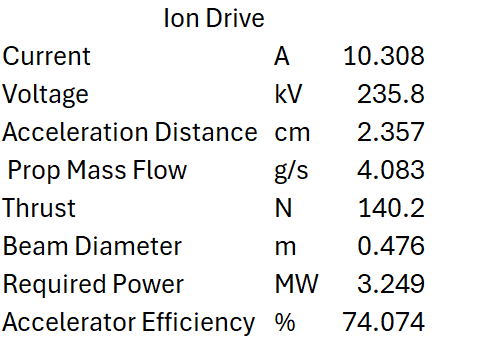
\includegraphics[width=.5\textwidth]{ion.png}
\end{figure}

\begin{figure}[hbt!]
    \centering
    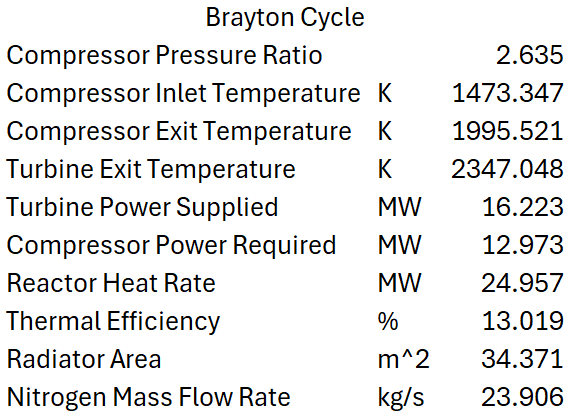
\includegraphics[width=.5\textwidth]{Brayton.png}
\end{figure}

\begin{figure}[hbt!]
    \centering
    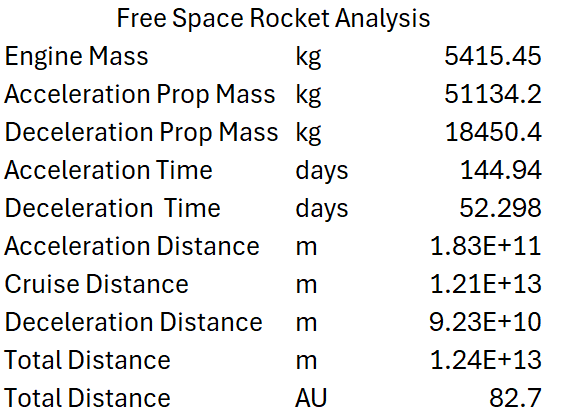
\includegraphics[width=.5\textwidth]{rocket.png}
\end{figure}



\pagebreak
\section*{Appendix A}

    
\end{document}
